% !TeX program = pdflatex
\documentclass[tikz,border=8pt]{standalone}
\usepackage{tikz}
\usetikzlibrary{angles,quotes,calc,positioning}
\definecolor{FigureBlue}{HTML}{2563EB}
\definecolor{FigureOrange}{HTML}{EA580C}
\begin{document}
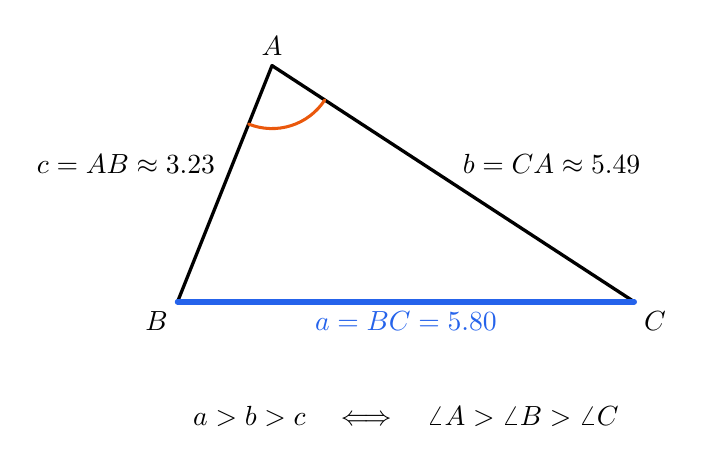
\begin{tikzpicture}[line cap=round,line join=round]
  \coordinate (A) at (1.2,3);
  \coordinate (B) at (0,0);
  \coordinate (C) at (5.8,0);
  \draw[line width=1.2pt] (A)--(B)--(C)--cycle;
  \draw[FigureBlue,line width=2pt] (B)--(C);
  \pic[draw=FigureOrange,line width=1.1pt,angle radius=8mm] {angle=B--A--C};
  \node[above] at (A) {$A$};\node[below left] at (B) {$B$};\node[below right] at (C) {$C$};
  \node[below,text=FigureBlue] at ($(B)!.5!(C)$) {$a=BC=5.80$};
  \node[above right] at ($(C)!.5!(A)$) {$b=CA\approx5.49$};
  \node[above left] at ($(A)!.5!(B)$) {$c=AB\approx3.23$};
  \node[below=12mm] at ($(B)!.5!(C)$) {$a>b>c\quad\Longleftrightarrow\quad \angle A>\angle B>\angle C$};
\end{tikzpicture}
\end{document}
